\documentclass[12pt]{article}
\usepackage{amsfonts}
\usepackage{amsthm}
\usepackage{amsmath}
\usepackage[mathscr]{euscript}
\usepackage{array}
\usepackage[thinlines]{easytable}
\usepackage{tikz}
\usepackage{pgfplots}
\usepackage[margin=2cm]{geometry}
\usepackage{graphicx}
\usepackage{xcolor}
\usepackage[utf8]{inputenc}
\usepackage[T1]{fontenc}
\usepackage[portuguese]{babel}
\usepackage{braket}
\usepackage{thmtools} 
\usepackage{hyperref}
\usepackage{environ}
\usepackage{enumitem}
\usepackage[backend=biber, style=numeric]{biblatex} %Imports biblatex package
\addbibresource{references.bib} %Import the bibliography file
%
\usepackage{lipsum} % Pode tirar esse :D

\graphicspath{.Images/}

\hypersetup{
	colorlinks=true,
	linkcolor=blue,
	filecolor=magenta,      
	urlcolor=cyan,
	pdftitle={Quântica Avançada - L1 - Lucas Froguel}
}


\def\be{\begin{equation}}
	\def\ee{\end{equation}}
\def\bee{\begin{equation*}}
	\def\eee{\end{equation*}}
\def\bea{\begin{eqnarray*}}
	\def\eea{\end{eqnarray*}}
\def\beaa{\begin{eqnarray}}
	\def\eeaa{\end{eqnarray}}

\def\f{\frac}
\def\del{\partial}

\def\R{\mathbb{R}}
\def\K{\mathbb{K}}
\def\C{\mathbb{C}}
\def\I{\mathbb{I}}
\def\Z{\mathbb{Z}}
\def\Q{\mathbb{Q}}
\def\N{\mathbb{N}}

\def\cd{\cdot}

\def\v#1{{\boldsymbol{#1}}}
\def\ve#1{\hat{\boldsymbol#1}}

\def\l{\left}
\def\r{\right}
\def\la{\l\langle}
\def\ra{\r\rangle}
\def\div{\nabla\cdot}
\def\curl{\nabla\times}
\def\grad{\nabla}
\def\lap{\nabla^2}

\def\s{\quad}
\def\ss{\qquad}
\def\infi{\infty}
\def\p{\partial}
\def\u{\cup}%union of two sets
\def\i{\cap}%intersection of two sets
\def\ds{\oplus}



\newtheorem{exercise}{Exercise}
\newtheorem{partinner}{Part}[exercise]

\newlist{exercises}{enumerate}{1}
\setlist[exercises]{wide = 0pt, listparindent=\parindent,labelsep = 0pt,leftmargin =\labelwidth}
\setlist[exercises, 1]{label =\itshape \bfseries Part~\arabic*.\; }

\newenvironment{answer}{\noindent\textbf{\textit{Answer.}} \normalfont }{\par\noindent\rule{\textwidth}{0.4pt}}
\NewEnviron{multianswer}[1][false]{%
	\ifthenelse{\equal{#1}{true}}%
	{\def\rulewidth{\textwidth}}%
	{\def\rulewidth{0.7\textwidth}}%
	\\ \noindent\textbf{\textit{Answer.}} \normalfont%
	\BODY%
	\par\noindent\rule{\rulewidth}{0.1pt}%
}


\newcommand\norm[1]{\left\lVert#1\right\rVert}

\DeclareMathOperator{\atan}{atan}
\DeclareMathOperator{\cotan}{cotan}
\DeclareMathOperator{\acos}{acos}
\DeclareMathOperator{\sech}{sech}
\DeclareMathOperator{\csch}{csch}
\DeclareMathOperator{\asinh}{asinh}
\DeclareMathOperator{\atanh}{atanh}
\DeclareMathOperator{\acoth}{acoth}
\DeclareMathOperator{\acosh}{acosh}
\DeclareMathOperator{\acsch}{acsch}
\DeclareMathOperator{\asech}{asech}
\DeclareMathOperator{\D}{D}
\DeclareMathOperator{\Tr}{tr}
\DeclareMathOperator{\Res}{Res}

\title{Mecânica Quântica Avançada \\ Lista 1}
\author{Lucas Froguel \\ IFT}
\date{}

\begin{document}
	\maketitle
	\listoftheorems[title={List of Exercises}]

	\begin{exercise}[4.4.1 - Dispersion and eigenvectors]
		Show that a necessary and sufficient condition for $|\psi\rangle$ to be an eigenvector of a Hermitian
		operator A is that the dispersion (4.8) $\Delta_\psi A = 0$.
	\end{exercise}
	\begin{answer}
		Vamos iniciar mostrando que se $\ket{\psi}=0$, então $\Delta_\psi A = 0$. Ora, por definição:
		\be
			\Delta_\psi A = \braket{\psi|A^2|\psi} - \braket{\psi|A|\psi}^2
		\ee
		É fácil ver que
		\be
			\braket{\psi|A^2|\psi} = \bra{\psi|A^\dagger}\ket{A|\psi} = a^2
		\ee
		E também
		\be
			\braket{\psi|A|\psi}^2 = \l(a\r)^2 = a^2
		\ee
		Logo, é trivial que $\Delta_\psi A = 0$. 
		
		Agora vamos assumir que a dispersão é nula, ou seja, $\Delta A = 0$. Então, por definição:		
		\begin{align}
			0 &= \sqrt{\langle A^2 \rangle - \langle A \rangle^2} \\
			\Rightarrow \langle A^2 \rangle &= \langle A \rangle^2
		\end{align}	
		Ora, considere
		\bea
			\braket{\psi|A^2|\psi} &=& \braket{\psi|A|\psi}^2 \\
			\braket{\psi|A^2|\psi} &=& \braket{\psi|A|\psi}\braket{\psi|A|\psi} \\
			A^2\ket{\psi} &=& \braket{\psi|A|\psi} A\ket{\psi} \\
			A\ket{\psi} &=& \braket{\psi|A|\psi} \ket{\psi} 
		\eea
		Logo, vemos que $\ket{\psi}$ é autovetor de $A$.
				
	\end{answer}

	\begin{exercise}[4.4.2 - The variational method]
		\begin{exercises}
			\item Let $\ket{\psi}$ be a vector (not normalized) in the Hilbert space of states and H be a Hamiltonian. The
			expectation value $\braket{H}_\psi$ is
			\be
				\braket{\psi}_\psi = \f{\braket{\psi|H|\psi}}{\braket{\psi|\psi}}
			\ee
			Show that if the minimum of this expectation value is obtained for $\ket{\psi}=\ket{\psi_m}$ and the maximum for $\ket{\psi}=\ket{\psi_M}$ , then
			\be
				H\ket{\psi_m} = E_m\ket{\psi_m}, \quad\quad H\ket{\psi_M} = E_M\ket{\psi_M}
			\ee 	
			where $E_m$ and $E_M$ are the smallest and largest eigenvalues.
			\begin{multianswer}
				É evidente que
				\be
					\braket{H}_{\psi_m} = \f{\braket{\psi_m|H|\psi_m}}{\braket{\psi_m|\psi_m}} = E_m
				\ee
				Portanto, é evidente que se $\braket{H}_{\psi_m}$ for mínimo, então $E_m$ também é. Vale um raciocínio análogo para $E_M=\braket{H}_{\psi_M}$. 		
			\end{multianswer}
	
			\item We assume that the vector $|\varphi\rangle$ depends on a parameter $\alpha:|\varphi\rangle=|\varphi(\alpha)\rangle$. Show that if
			\begin{equation}
				\frac{\partial\braket{H}_{\varphi(\alpha)}}{\partial \alpha}\bigg|_{\alpha=\alpha_0}=0,
			\end{equation}
			then $E_{m} \leq\langle H\rangle_{\varphi\left(\alpha_{0}\right)}$ if $\alpha_{0}$ corresponds to a minimum of $\langle H\rangle_{\varphi(\alpha)}$, and $\langle H\rangle_{\varphi\left(\alpha_{0}\right)} \leq E_{M}$ if $\alpha_{0}$ corresponds to a maximum. This result forms the basis of an approximation method called the variational method (Section 14.1.4).
		\begin{multianswer}
			Vamos abrir a derivada:
			\be
				\frac{\partial\braket{H}_{\varphi(\alpha)}}{\partial \alpha} = \f{1}{\braket{\psi|\psi}}\l( \bra{\psi|H} \partial_\alpha\ket{\psi} + (\partial_\alpha\bra{\psi})\ket{H|\psi}\r) - \f{\braket{\psi|H|\psi}}{\braket{\psi|\psi}^2}\l( (\partial_\alpha\bra{\psi})\ket{\psi} + \bra{\psi}\partial_\alpha\ket{\psi}\r) 
			\ee
			Então, em $\alpha_0$
			\be
				\braket{\psi|H|\partial_\alpha\psi} + \braket{\partial_\alpha\psi|H|\psi} = \f{\braket{\psi|H|\psi}}{\braket{\psi|\psi}}\big( \braket{\partial_\alpha\psi|\psi} + \braket{\psi|\partial_\alpha\psi}\big)
			\ee
			Isolando a quantidade de interesse:
			\be
				\braket{H}_{\varphi(\alpha_0)} = \f{\braket{\psi|H|\partial_\alpha\psi} + \braket{\partial_\alpha\psi|H|\psi}}{\braket{\partial_\alpha\psi|\psi} + \braket{\psi|\partial_\alpha\psi}}
			\ee 
			Podemos reescrever, usando que $H=H^\dagger$:
			\be
				\braket{H}_{\varphi(\alpha_0)} = \f{\braket{\partial_\alpha\psi|H|\psi}^\dagger + \braket{\partial_\alpha\psi|H|\psi}}{\braket{\partial_\alpha\psi|\psi}^\dagger + \braket{\partial_\alpha\psi|\psi}}
			\ee
			
			Podemos expandir qualquer estado usando os autokets do hamiltoniano, que são ortonormais:
			\be
				\ket{\psi} = \sum c_j\ket{\psi_j}
			\ee
			De modo que
			\be
				\partial_\alpha\ket{\psi} = \sum \f{\partial c_j}{\partial\alpha} \ket{\psi_j}
			\ee
			Assim, vale que
			\be
				\braket{\partial_\alpha\psi|\psi} = \sum c_j\f{\partial c_j^*}{\partial\alpha}
			\ee
			E também
			\be
				\braket{\partial_\alpha\psi|H|\psi} = \sum E_jc_j\f{\partial c_j^*}{\partial\alpha}
			\ee
			Considere o denominador:
			\bea
				\braket{\partial_\alpha\psi|\psi}^\dagger + \braket{\partial_\alpha\psi|\psi} 
					&=& \sum c_j \f{\partial c_j^*}{\partial\alpha} + c_j^*\f{\partial c_j}{\partial\alpha} \\
					&=& \sum \f{\partial}{\partial\alpha} (c_j^*c_j) \\
					&=& \sum \partial_\alpha |c_j|^2 \\
					&=& \partial_\alpha \sum |c_j|^2
			\eea
			Considerando, enfim, o numerador e fazendo os mesmos cálculos:
			\bea
				\braket{\partial_\alpha\psi|H|\psi}^\dagger + \braket{\partial_\alpha\psi|H|\psi} 
					&=& \sum E_jc_j\f{\partial c_j^*}{\partial\alpha} + E_j c_* \f{\partial c_j}{\partial\alpha} \\
					&=& \sum E_j \partial_\alpha |c_j|^2 \\
					&=& \partial_\alpha \sum E_j|c_j|^2 
			\eea
			É óbvio, então, que
			\be
				E_m \partial_\alpha\sum |c_j|^2 \leq \partial_\alpha\sum E_j|c_j|^2 \leq E_M \partial_\alpha\sum |c_j|^2
			\ee 
			Portanto, concluímos que
			\be
				E_m \leq \braket{H}_{\varphi(\alpha_0)} \leq E_M
			\ee	
		\end{multianswer}
	
	% Part 3
		\item If $H$ acts in a two-dimensional space, its most general form is
		$$
		H=\left(\begin{array}{cc}
			a+c & b \\
			b & a-c
		\end{array}\right),
		$$
		where $b$ can always be chosen to be real. Parametrizing $|\varphi(\alpha)\rangle$ as
		
		$$
		|\varphi(\alpha)\rangle=\left(\begin{array}{c}
			\cos \alpha / 2 \\
			\sin \alpha / 2
		\end{array}\right)
		$$
		find the values of $\alpha_{0}$ by seeking the extrema of $\langle\varphi(\alpha)|H| \varphi(\alpha)\rangle$. Rederive (2.35).
		\begin{multianswer}[true]
			Começamos considerando a equação do valor médio explicitamente:
			\bea
				\braket{\psi|H|\psi} 
					&=& 
					\begin{bmatrix}
						\cos(\alpha/2) & \sin(\alpha/2)
					\end{bmatrix}
					\begin{bmatrix}
						a+c & b \\
						b & a-c
					\end{bmatrix}
					\begin{bmatrix}
						\cos(\alpha/2) \\
						\sin(\alpha/2)
					\end{bmatrix} \\
					&=& 
					\begin{bmatrix}
						\cos(\alpha/2) & \sin(\alpha/2)
					\end{bmatrix}
					\begin{bmatrix}
						(a+c)\cos(\alpha/2) + b\sin(\alpha/2) \\
						b\cos(\alpha/2) + (a-c)\sin(\alpha/2)
					\end{bmatrix} \\
					&=& 
					(a+c)\cos^2(\alpha/2) + b\sin(\alpha/2)\cos(\alpha/2) + b\cos(\alpha/2)\sin(\alpha/2) + (a-c)\sin^2(\alpha/2) \\
					&=& 
					a(\sin^2(\alpha/2)+ \cos^2(\alpha/2)) + c(\cos^2(\alpha/2) - \sin^2(\alpha/2)) + b\sin(\alpha) \\
					&=& a + b\sin(\alpha) + c\cos(\alpha)
			\eea
			Vejamos os extremos dessa função:
			\bea	
				\partial_\alpha \braket{\psi|H|\psi} &=& b\cos(\alpha) - c\sin(\alpha) = 0 \\
				b\cos(\alpha) &=& c\sin(\alpha) \\
				\tan(\alpha) &=& b/c \\
				\alpha_0 &=& \atan(b/c)
			\eea
			A Eq.(2.35) se refere aos autovetores e autovalores de $H$. Vejamos o caso do nosso $\psi$:
			\bea	
				H\ket{\psi} &=& 
				\l( a\begin{bmatrix}
					  1 & 0 \\
					  0 & 1
					\end{bmatrix}
					+ \sqrt{b^2+c^2}
					\begin{bmatrix}
						\cos\alpha & \sin\alpha \\
						\sin\alpha & -\cos\alpha
					\end{bmatrix}
				\r)
				\begin{bmatrix}
					\cos(\alpha/2) \\
					\sin(\alpha/2)
				\end{bmatrix} \\
				&=& 
				a\begin{bmatrix}
					\cos(\alpha/2) \\
					\sin(\alpha/2)
				\end{bmatrix} 
				+ 
				\sqrt{b^2+c^2}
				\begin{bmatrix}
					\cos\alpha\cos(\alpha/2) + \sin\alpha\sin(\alpha/2) \\
					\sin\alpha\cos(\alpha/2) - \cos\alpha\sin(\alpha/2)
				\end{bmatrix} \\
				&=& 
				a + \sqrt{b^2+c^2} 
				\begin{bmatrix}
					\cos(\alpha/2) \\
					\sin(\alpha/2)
				\end{bmatrix} 
			\eea
			onde usamos a Eq.(2.34) e algumas identidades trigonométricas.	
		\end{multianswer}
	\end{exercises}
	\end{exercise}

	\begin{exercise}[4.4.3 - The Feynman-Hellmann theorem]
		Let a Hamiltonian $H$ depend on a parameter $\lambda: H=H(\lambda)$. Let $E(\lambda)$ be a nondegenerate eigenvalue and $|\varphi(\lambda)\rangle$ be the corresponding normalized eigenvector $\left(\|\varphi(\lambda)\|^{2}=1\right)$ :
		
		$$
		H(\lambda)|\varphi(\lambda)\rangle=E(\lambda)|\varphi(\lambda)\rangle
		$$
		Demonstrate the Feynman-Hellmann theorem:
		$$
		\frac{\partial E}{\partial \lambda}=\left\langle\varphi(\lambda)\left|\frac{\partial H}{\partial \lambda}\right| \varphi(\lambda)\right\rangle .
		$$
	\end{exercise}
	\begin{answer}
		Sabemos que podemos escrever
		\be
			E(\lambda) = \braket{\psi|H|\psi}
		\ee
		Então considere:
		\be
			\partial_\lambda E = \braket{\partial_\lambda\psi|H|\psi} + \braket{\psi|\partial_\lambda|\psi} + \braket{\psi|H|\partial_\lambda\psi} 
		\ee
		Logo, é suficiente mostrar que 
		\be
			\braket{\partial_\lambda\psi|H|\psi} +  \braket{\psi|H|\partial_\lambda\psi} = 0
		\ee
		Considere:
		\bea
			\braket{\partial_\lambda\psi|H|\psi} +  \braket{\psi|H|\partial_\lambda\psi} 
			&=& \braket{\partial_\lambda\psi|E|\psi} + \braket{\psi|E^\dagger|\partial_\lambda\partial_\lambda\psi} \\
 			&=& E \l(\braket{\partial_\lambda\psi|\psi} + \braket{\psi|\partial_\lambda\psi}\r) \\ 
			&=& E( \partial_\lambda\braket{\psi|\psi}) \\
			&=& E\partial_\lambda 1 \\
			&=& 0
		\eea
		onde usamos o fato de $H$ ser hermitiano e ter autovalores reais e de $\ket{\psi}$ ser normalizado. Portanto, fica demonstrado o teorema.		
	\end{answer}

	\begin{exercise}[4.4.4 - Time evolution of a two-level system]
		We consider a two-level system with Hamiltonian $H$ represented by the matrix
		$$
		H=\hbar\left(\begin{array}{cc}
			A & B \\
			B & -A
		\end{array}\right)
		$$
		in the basis
		$$
		|+\rangle=\left(\begin{array}{l}
			1 \\
			0
		\end{array}\right), \quad|-\rangle=\left(\begin{array}{l}
			0 \\
			1
		\end{array}\right)
		$$
		According to (2.35), the eigenvalues and eigenvectors of $H$ are
		$$
		\begin{array}{ll}
			E_{+}=\hbar \sqrt{A^{2}+B^{2}}, & \left|\chi_{+}\right\rangle=\cos \frac{\theta}{2}|+\rangle+\sin \frac{\theta}{2}|-\rangle \\
			E_{-}=-\hbar \sqrt{A^{2}+B^{2}}, & \left|\chi_{-}\right\rangle=-\sin \frac{\theta}{2}|+\rangle+\cos \frac{\theta}{2}|-\rangle
		\end{array}
		$$
		with
		$$
		A=\sqrt{A^{2}+B^{2}} \cos \theta, \quad B=\sqrt{A^{2}+B^{2}} \sin \theta, \quad \tan \theta=\frac{B}{A}
		$$
		\begin{exercises}
		% Part 1
		\item The state vector $|\varphi(t)\rangle$ at time $t$ can be decomposed on the $\{|+\rangle,|-\rangle\}$ basis:
		
		$$
		|\varphi(t)\rangle=c_{+}(t)|+\rangle+c_{-}(t)|-\rangle
		$$
		
		Write down the system of coupled differential equations which the components $c_{+}(t)$ and $c_{-}(t)$ satisfy.
		\begin{multianswer}
				Começamos escrevendo:
				\be
					\ket{\varphi(t)} = \begin{pmatrix}
						c_+(t) \\ c_-(t)
						\end{pmatrix}
				\ee
				Agora montamos a equação de Schrödinger:
				\bea
					H\ket{\varphi(t)} &=& -i\hbar \partial_t\ket{\varphi(t)} \\
					\hbar\begin{pmatrix}
						A & B \\
						B & -A
					\end{pmatrix} 
					\begin{pmatrix}
						c_+(t) \\ c_-(t)
					\end{pmatrix} 
					&=& 
					-i\hbar 
					\begin{pmatrix}
						\partial_t c_+(t) \\ \partial_t c_-(t)
					\end{pmatrix} \\
					\begin{pmatrix}
						Ac_+ + Bc_- \\ Bc_+ - Ac_-
					\end{pmatrix}
					&=&
					-i \begin{pmatrix}
						\dot{c}_+(t) \\ \dot{c}_-(t)
					\end{pmatrix}
				\eea
			Ou seja, temos as equações diferenciais:
			\beaa
				i\dot{c}_+ &=& Ac_+ + Bc_- \\
				i\dot{c}_- &=& Bc_+ - Ac_-
			\eeaa				
		\end{multianswer}
		
		\item Let $|\varphi(t=0)\rangle$ be decomposed on the $\left\{\left|\chi_{+}\right\rangle,\left|\chi_{-}\right\rangle\right\}$basis:
		$$
		|\varphi(t=0)\rangle=|\varphi(0)\rangle=\lambda\left|\chi_{+}\right\rangle+\mu\left|\chi_{-}\right\rangle, \quad|\lambda|^{2}+|\mu|^{2}=1
		$$
		Show that $c_{+}(t)=\langle+\mid \varphi(t)\rangle$ is written as
		$$
		c_{+}(t)=\lambda \mathrm{e}^{-\mathrm{i} \Omega t / 2} \cos \frac{\theta}{2}-\mu \mathrm{e}^{\mathrm{i} \Omega t / 2} \sin \frac{\theta}{2}
		$$
		with $\Omega=2 \sqrt{A^{2}+B^{2}}$. Here $\hbar \Omega$ is the energy difference of the two levels. Show that $c_{+}(t)$ (as well as $\left.c_{-}(t)\right)$ satisfies the differential equation
		$$
		\ddot{c}_{+}(t)+\left(\frac{\Omega}{2}\right)^{2} c_{+}(t)=0 .
		$$
		\begin{multianswer}
			Vamos começar pela segunda parte, mostrando a validez da equação diferencial. Considere as EDOs que obtemos e vamos deriva-las mais uma vez (faremos as contas para $c_+$, pois são análogas para $c_-$.):
			\be
				i\ddot{c}_+ = A\dot{c}_+ + B\dot{c}_-
			\ee
			Mas note, também, que:
			\bea
				A\dot{c}_+ &=& -iA^2c_+ - iABc_- \\
				B\dot{c}_- &=& -iB^2c_+ + iABc_-
			\eea
			Logo, 
			\be
				A\dot{c}_+ + B\dot{c}_- = -i(A^2+B^2)c_+
			\ee
			Portanto,
			\be
				i\ddot{c}_+ = -i(A^2+B^2)c_+
			\ee
			que, simplificando, implica na expressão desejada
			\be
				\ddot{c}_+ +\l(\f{\Omega}{2}\r)^2c_+ = 0
			\ee
			Vamos considerar agora a outra parte. Sabemos que
			\be
				\ket{\psi_t} = \hat{U}\ket{\psi_0}
			\ee
			onde $\hat{U}$ é o operador de evolução temporal. Assim, usando a base dos autoestados de $\hat{H}$:
			\bea
				\ket{\psi_t} &=& \hat{U}\ket{\psi_0} \\
							&=& e^{-i\hat{H}t/\hbar} \l(\lambda\left|\chi_{+}\right\rangle+\mu\left|\chi_{-}\right\rangle\r) \\
							&=& \lambda e^{-iE_+t/\hbar}\ket{\chi_+} + \mu e^{iE_-t/\hbar}\ket{\chi_-}
			\eea
			Abrindo agora na base natural:
			\be
				\ket{\psi_t} = \lambda e^{-iE_+t/\hbar}\l(\cos \frac{\theta}{2}|+\rangle+\sin \frac{\theta}{2}|-\rangle\r) + \mu e^{iE_-t/\hbar}\l(-\sin \frac{\theta}{2}|+\rangle+\cos \frac{\theta}{2}|-\rangle\r)
			\ee
			Por fim, calculamos $c_+(t) = \braket{+|\psi_t}$ e usamos $\Omega = 2E_\pm$:
			\be
				c_+(t) = \lambda \mathrm{e}^{-\mathrm{i} \Omega t / 2} \cos \frac{\theta}{2}-\mu \mathrm{e}^{\mathrm{i} \Omega t / 2} \sin \frac{\theta}{2}
			\ee
			
			
		\end{multianswer}
		
		% Part 3
		\item We assume that $c_{+}(0)=0$. Find $\lambda$ and $\mu$ up to a phase as well as $c_{+}(t)$. Show that the probability of finding the system in the state $|+\rangle$ at time $t$ is
		
		$$
		\mathrm{p}_{+}(t)=\sin ^{2} \theta \sin ^{2}\left(\frac{\Omega t}{2}\right)=\frac{B^{2}}{A^{2}+B^{2}} \sin ^{2}\left(\frac{\Omega t}{2}\right) .
		$$
		\begin{multianswer}[true]
			Se $c_+(0)=0$, então precisa ser que
			\be
				 \lambda\cos(\theta/2) - \mu\sin(\theta/2) = 0
			\ee
			Logo, é verdade que
			\be
				\lambda = \mu \tan(\theta/2)
			\ee
			Mas, pela normalização:
			\bea
				|\lambda|^2 + |\mu|^2 &=& 1 \\
				|\mu\tan(\theta/2)|^2 + |\mu|^2 &=& 1 \\
				|\mu|^2|\tan(\theta/2)|^2 + |\mu|^2 &=& \\
				|\mu|^2 &=& \f{1}{1 + |\tan(\theta/2)|^2}
			\eea
			Logo, a menos de uma fase $e^{ia}$, 
			\bea
				\mu =  &=& \f{1}{\sqrt{1 + |\tan(\theta/2)|^2}} \\
				\lambda  &=& \f{\tan(\theta/2)}{\sqrt{1 + |\tan(\theta/2)|^2}}
			\eea
			Vamos supor, daqui em diante, $\theta\in[0, \pi]$ para tirarmos a tangente do módulo. Usando a solução geral de $c_+(t)$, basta usarmos os valores calculados de $\lambda$ e $\mu$:
			\bea
				c_+(t) &=& \l(\f{\tan(\theta/2)}{\sqrt{1 + \tan(\theta/2)^2}}\r) \mathrm{e}^{-\mathrm{i} \Omega t / 2} \cos \frac{\theta}{2}-\l( \f{1}{\sqrt{1 + \tan(\theta/2)^2}}\r) \mathrm{e}^{\mathrm{i} \Omega t / 2} \sin \frac{\theta}{2} \\
					&=& \f{\sin(\theta/2)}{\sqrt{1+\tan^2(\theta/2)}}\l( e^{-i\Omega t/2} - e^{i\Omega t/2}\r) \\
					&=& \f{-2i\sin(\theta/2)}{\sqrt{1+\tan^2(\theta/2)}} \sin\l(\f{\Omega t}{2}\r)
			\eea 
			Ora, tendo isso, a probabilidade é $p(t)=|c(t)|^2$. Portanto, considere:
			\bea
				p(t) &=& |c(t)|^2 \\
					&=& |c^2(t)| \\
					&=& \f{2\sin^2(\theta/2)}{1+\tan^2(\theta/2)} \sin^2(\Omega t/2)
			\eea
			Aqui notamos que:
			\be
				1+\tan^2(\theta/2) = 1 + \f{\sin^2(\theta/2)}{\cos^2(\theta/2)} = \f{\sin^2(\theta/2) + \cos^2(\theta/2)}{\cos^2(\theta/2)} = \f{1}{\cos^2(\theta/2)}
			\ee
			Então, é fácil ver que
			\be
				p(t) = \sin^2(\theta)\sin^2(\Omega t/2)
			\ee
			E ainda podemos escrever
			\be
				c_+(t) = -i\sin(\theta)\sin(\Omega t/2)
			\ee
		\end{multianswer}
		\end{exercises}
	\end{exercise}
	
	\begin{exercise}[4.4.5 - Unstable states]
		Let $|\varphi(0)\rangle$ represent the state vector at time $t=0$ of an unstable particle, or more generally that of an unstable quantum state such as an atom in an excited state, and let $\mathrm{p}(t)$ be the probability (survival probability) that it has not decayed at time $t$. The particle is assumed to be isolated from external influences (but not from quantized fields), so that the Hamiltonian $H$ that governs the decay is time-independent. Let $|\Psi(t)\rangle$ be the state vector at time $t$ of the full quantum system
		$$
		|\Psi(t)\rangle=\exp \left(-\frac{i H t}{\hbar}\right)|\varphi(0)\rangle .
		$$
		The probability amplitude for finding the state of the quantum system at time $t$ in $|\varphi(0)\rangle$ is
		$$
		c(t)=\langle\varphi(0) \mid \Psi(t)\rangle=\left\langle\varphi(0)\left|\exp \left(-\frac{\mathrm{i} H t}{\hbar}\right)\right| \varphi(0)\right\rangle
		$$
		and the survival probability is
		$$
		\mathrm{p}(t)=|c(t)|^{2}=|\langle\Psi(t) \mid \varphi(0)\rangle|^{2}=\langle\Psi(t)|\mathcal{P}| \Psi(t)\rangle
		$$
		where $\mathcal{P}=|\varphi(0)\rangle\langle\varphi(0)|$ is the projector on the initial state.
		\begin{exercises}
			% Part 1
			\item Let us first restrict ourselves to very short times. Show that for $t \rightarrow 0$
			$$
			\mathrm{p}(t) \simeq 1-\frac{(\Delta H)^{2}}{\hbar^{2}} t^{2}
			$$
			so that, for very short times, the decay law is certainly not exponential. The expectation values of $H$ and $H^{2}$ are computed in the state $|\varphi(0)\rangle$. Note that $\Delta H$ must be finite, otherwise $|\varphi(0)\rangle$ would not belong to the domain of $H^{2}$, which would be difficult to imagine physically (see Chapter 7 for the definition of the domain of an operator).
			\begin{multianswer}
				Começamos lembrando que
				\be
					(\Delta H)^2 = \braket{H^2} - \braket{H}^2
				\ee
				Para $t\to0$, podemos aproximar
				\be
					e^{-iHt/\hbar} \approx 1 -\f{iHt}{\hbar} - \f{H^2t^2}{2\hbar^2}
				\ee
				Logo, 
				\bea
					c(t) &=& \braket{\phi_0 | 1 - \f{iHt}{\hbar} - \f{H^2t^2}{2\hbar^2} | \phi_0} \\
						&=& \braket{\phi_0|\phi_0} - \f{it}{\hbar}  \braket{H} - \f{t^2\braket{H^2}}{2\hbar^2}\\
						&=& 1 - \f{it\braket{H}}{\hbar} - \f{t^2\braket{H^2}}{2\hbar^2}
				\eea
				Portanto,
				\bea
					p(t) &=& |c(t)|^2 \\
						&=& 1  - \f{t^2\braket{H^2}}{\hbar^2}  + \f{t^2\braket{H}^2}{\hbar^2} + \f{t^4\braket{H^2}^2}{\hbar^4} \\
						&=& 1 - \f{t^2}{\hbar^2}\l(\braket{H^2}  - \braket{H}^2 \r) + \mathcal{O}(t^4)  \\
						&=& 1 - \f{t^2(\Delta H)^2}{\hbar^2}
				\eea
				como queríamos mostrar. 
			\end{multianswer}
		
			% Part 2
			\item A more general result is obtained as follows. Show first that
			$$
			\Delta \mathcal{P}^{2}=\langle\mathcal{P}\rangle-\langle\mathcal{P}\rangle^{2}
			$$
			and use (4.27) to deduce the inequality $\left(\Delta H=\left(\left\langle H^{2}\right\rangle-\langle H\rangle^{2}\right)^{1 / 2}\right)$
			$$
			\left|\frac{\mathrm{d} \mathrm{p}(t)}{\mathrm{d} t}\right| \leq \frac{2 \Delta H}{\hbar} \sqrt{\mathrm{p}(1-\mathrm{p})}
			$$
			Integrating this differential equation, derive
			$$
			\mathrm{p}(t) \geq \cos ^{2}\left(\frac{t \Delta H}{\hbar}\right) \quad 0 \leq t \leq \frac{\pi \hbar}{2 \Delta H}
			$$		
			\begin{multianswer}
				Sabemos que $\mathcal{P} = \ket{\psi_0}\bra{\psi_0}$. Assim, como $\mathcal{P}$ é um projetor, é trivial que seja idempotente:
				\be
					\mathcal{P}^2 = \l(\ket{\psi_0}\bra{\psi_0}\r)\l(\ket{\psi_0}\bra{\psi_0}\r) = \ket{\psi_0}\braket{\psi_0|\psi_0}\bra{\psi_0} = \ket{\psi_0}\bra{\psi_0} = \mathcal{P}
				\ee
				À partir disso, decorre diretamente a propriedade de:
				\be
					(\Delta\mathcal{P})^2 = \braket{\mathcal{P}} - \braket{\mathcal{P}}^2
				\ee
				A Eq.(4.27) diz que
				\be
					\Delta_{\varphi} H \Delta_{\varphi} A \geq \frac{1}{2}\left|\langle[A, H]\rangle_{\varphi}\right|=\frac{1}{2} \hbar\left|\frac{\mathrm{d}}{\mathrm{d} t}\langle A\rangle_{\varphi}(t)\right|
				\ee
				onde, no nosso caso, teremos $A=\mathcal{P}$. Usando $p(t)=\braket{\mathcal{P}}$ e aplicando para o nosso caso:
				\be
					\l|\f{dp}{dt}\r| \leq \f{2\Delta H}{\hbar}\Delta\mathcal{P} 
				\ee
				Então, basta escrever $\Delta\mathcal{P}$ na forma desejada. Ora, isso é fácil, pois
				\bea
					\Delta\mathcal{P} &=& \sqrt{\braket{\mathcal{P}} - \braket{\mathcal{P}}^2} \\
							&=& \sqrt{p - p^2} \\
							&=& \sqrt{p(1-p)}
				\eea
				Portanto, 
				\be
					\l|\f{dp}{dt}\r| \leq \f{2\Delta H}{\hbar}\sqrt{p(1-p)} 
				\ee
				Vamos, agora, integrar essa inequação:
				\bea
					\f{dp}{\sqrt{p(1-p)}} &\leq& \f{2\Delta H}{\hbar} dt  \\
					\int \f{dp}{\sqrt{p(1-p)}} &\leq& \int \f{2\Delta H}{\hbar} dt = \f{2t\Delta H}{\hbar}
				\eea
				Vejamos o lado esquerdo com mais cuidado. Vamos usar a substituição $u=\sqrt{p}$, onde $2du = dp/\sqrt{p}$. Assim, 
				\be
					\int \f{dp}{\sqrt{p(1-p)}} = \int \f{2du}{\sqrt{1-u^2}} = 2\acos(u)
				\ee
				Agora, notamos que isso implica
				\be
					0 \leq \f{2t\Delta H}{\hbar} \leq \pi
				\ee
				Ou,
				\be
					0 \leq t \leq \frac{\pi \hbar}{2 \Delta H}
				\ee
				Voltando à inequação das integrais e usando que $u=\sqrt{p}$. 
				\bea
					\acos(u) &\leq& \f{t\Delta H}{\hbar} \\ 
					\sqrt{p} &\geq& \cos\l(\f{t\Delta H}{\hbar}\r)  \\
					p(t) &\geq& \cos^2\l(\f{t\Delta H}{\hbar}\r) 
				\eea
				o sinal da inegualdade muda, pois $\cos(x)$ decresce no intervalo $x\in[0, \pi]$. 	
			\end{multianswer}
		
			% Part 3
			\item Let $|n\rangle$ be a complete set of eigenstates of the Hamiltonian
			$$
			H|n\rangle=E_{n}|n\rangle
			$$
			Show that $c(t)$ is given by the Fourier transform of a spectral function $w(E)$
			$$
			w(E)=\sum_{n}|\langle n \mid \varphi(0)\rangle|^{2} \delta\left(E-E_{n}\right)
			$$
			Set $E_{0}=\langle H\rangle$ and give the expression of $(\Delta H)^{2}$ in terms of $w(E)$ and $E_{0}$.
			\begin{multianswer}
				Por definição,
				\be
					c(t)=\braket{\varphi(0) | \Psi(t)}
				\ee
				com
				\be
					|\Psi(t)\rangle=\exp\left(-\frac{i H t}{\hbar}\right)|\varphi(0)\rangle
				\ee
				Vamos considerar $c(t)$ na base das autoenergias:
				\bea
					\ket{\Psi(t)} &=& \exp\left(-\frac{i H t}{\hbar}\right) \sum_{n} \braket{n|\psi_0}\ket{n} \\
						&=& \sum_n \braket{n|\psi_0} e^{-iE_nt/\hbar} \ket{n}
				\eea
				Logo, sendo 
				\be
					\bra{\psi_0} = \sum_k \braket{\psi_0|k}\bra{k}
				\ee
				Vale que
				\bea
					c(t) &=& \braket{\psi_0|\Psi_t} \\
						&=& \l(\sum_k \braket{\psi_0|k}\bra{k}\r)\l( \sum_n \braket{n|\psi_0} e^{-iE_nt/\hbar} \ket{n}\r) \\
						&=& \sum_{n, k} \braket{\psi_0|k} \braket{n|\psi_0} e^{-iE_nt/\hbar} \braket{k|n} \\
						&=& \sum_{n, k} \braket{\psi_0|k} \braket{n|\psi_0} e^{-iE_nt/\hbar} \delta(n-k) \\
						&=& \sum_n |\braket{\psi_0|n}|^2e^{-iE_nt/\hbar}
				\eea
				Aqui nós observamos que a transformada de fourier da delta de dirac é:
				\be
					\int_{-\infty}^{\infty} \delta(E-E_n) e^{-2\pi i tE} dE = e^{-2\pi i tE_n}
				\ee
				da onde é óbvio a transformada inversa da exponencial que temos em mão. Portanto,
				\bea
				\omega(E) &=& \mathcal{F}^{-1} \l( \sum_n |\braket{\psi_0|n}|^ 2e^{-iE_nt/\hbar}\r) \\
					&=&  \sum_n |\braket{\psi_0|n}|^2 \mathcal{F}^{-1}\l(e^{-iE_nt/\hbar}\r) \\
					&=& \sum_n |\braket{\psi_0|n}|^2 \delta(E-E_n)
				\eea
				como queríamos mostrar. Agora, seja $E_0=\braket{H}$. Sabemos que
				\be
					(\Delta H)^2 = \braket{H^2} - \braket{H}^2 
				\ee
				Ademais, por uma conta análoga à que fizemos para calcular $c(t)$:
				\bea
					\braket{H} &=& \braket{\psi_0 | H | \psi_0} \\
						&=& \sum_n E_n |\braket{\psi_0|n}|^2 \\
						&=& \int E\omega(E) dE
				\eea
				E
				\bea
					\braket{H^2} &=& \braket{\psi_0 | H^2 | \psi_0} \\
					&=& \sum_n E_n^2 |\braket{\psi_0|n}|^2 \\
					&=& \int E^2\omega(E) dE
				\eea
				Ambas as integrais são facilmente checadas substituindo $\omega(E)$ e notando o efeito da $\delta(E-E_n)$ de matar a integral. Portanto, podemos escrever
				\be
					(\Delta H)^2 = \int E(E - E_0)\omega(E) dE
				\ee
				
			\end{multianswer}
		
			% Part 4
			\item If $w(E)$ has a Lorentzian shape
			$$
			w(E)=\frac{\Gamma \hbar}{2 \pi} \frac{1}{\left(E-E_{0}\right)^{2}+\hbar^{2} \Gamma^{2} / 4}
			$$
			show that
			$$
			c(t)=\mathrm{e}^{-\mathrm{i} E_{0} t / \hbar} \mathrm{e}^{-\Gamma t / 2}
			$$
			and that the decay law is an exponential. The width of $w(E)$ is $\hbar \Gamma$, but $\Delta H$ is infinite, Thus $\Delta H$ is a rather poor measure of energy spread, and the width $\hbar \Gamma=\Delta E$ is the physically relevant quantity.
			\begin{multianswer}[true]
				Iremos realizar a transformada de Fourier dessa função:
				\bea
					c(t) &=& \mathcal{F}\l(\omega(E)\r) \\
						&=&  \int_{-\infty}^{\infty} \frac{\Gamma \hbar}{2 \pi} \frac{e^{-2i\pi tE}}{\left(E-E_{0}\right)^{2}+\hbar^{2} \Gamma^{2} / 4} dE \\
						&=& \f{\Gamma\hbar}{2\pi}e^{-2i\pi tE_0} \int_{-\infty}^{\infty} \frac{e^{-2i\pi t(E-E_0)}}{\left(E-E_{0}\right)^{2}+\hbar^{2} \Gamma^{2} / 4} dE 
				\eea
				Agora iremos considerar um contorno adequado e a versão complexa dessa integral. Se usarmos o contorno que cobre o UHP (upper half plane), podemos escrever:
				\be
					\int_{-\infty}^{\infty} \frac{e^{-2i\pi t(E-E_0)}}{\left(E-E_{0}\right)^{2}+\hbar^{2} \Gamma^{2} / 4} dE  = \oint \f{e^{-2i\pi tz}}{z^2 + k^2} dz
				\ee
				onde $k=\hbar\Gamma/2$ e $z=E-E_0$. Os polos dessa função ocorrem em $z_\pm=\pm ik$ e são de primeira ordem. Como apenas $z_+=ik$ está no UHP e a função é, no resto, analítica, podemos calcular a integral usando o teorema dos resíduos. Ora, o resíduo é
				\bea
					\Res(f)_{z_+} &=& \lim_{z\to z_+} \f{e^{-2i\pi tz}}{(z-ik)(z+ik)} (z-ik) \\ 
							&=& \f{e^{-2i\pi t (ik)}}{2ik} \\
							&=& \f{e^{2\pi tk}}{2ik}
				\eea
				Logo,
				\bea
					\oint \f{e^{-2i\pi tz}}{z^2 + k^2} dz &=& 2\pi i \sum_{z\in\text{UHP}} \Res(f)_z \\
						&=& \l(\f{\pi}{k}\r) e^{2\pi tk} \\
						&=& \l(\f{2\pi}{\hbar\Gamma}\r) e^{\pi\hbar\Gamma t}
				\eea
				Portanto,
				\be
					c(t) = e^{-2\pi i tE_0}e^{\pi \hbar\Gamma t}
				\ee
				
				
				
				*
				
			\end{multianswer}
		\end{exercises}
	\end{exercise}

	\begin{exercise}[4.4.6 - The solar neutrino puzzle] \label{ex4.4.6}
		The nuclear reactions occurring in the interior of the Sun produce an abundance of electron neutrinos $\nu_{\mathrm{e}} ; 95 \%$ of these are produced in the reaction
		$$
		\mathrm{p}+\mathrm{p} \rightarrow{ }^{2} \mathrm{H}+\mathrm{e}^{+}+\nu_{\mathrm{e}}
		$$
		The Earth receives $6.5 \times 10^{14}$ neutrinos per second and per square metre from the Sun. For about thirty years several experiments sought to detect these neutrinos, but all of them concluded that the measured neutrino flux is only about half the flux calculated using the standard solar model. Now this model is considered to be quite reliable, in particular owing to recent results from helioseismology. In any case, the uncertainties in the solar model cannot explain this "solar neutrino deficit." The combined results of three experiments (see Footnote 4, Chapter 1) have now shown with no possible doubt that this neutrino deficit is due to the transformation of $\nu_{\mathrm{e}}$ neutrinos into other types of neutrino during the passage from the Sun to the Earth. These experiments show that the total neutrino flux predicted by the solar model is correct, but that the measured electron neutrino flux is too small. We shall construct a simplified theory which gives the essential physics. We assume that
		\begin{itemize}
			\item there exist only two types of neutrino, the electron neutrino $\nu_{\mathrm{e}}$ and the muon neutrino $v_{\mu}$ (in fact, there is also a third type, the $\tau$ neutrino $\nu_{\tau}$ );
		
			\item the entire phenomenon takes place in a vacuum during the propagation from the Sun to the Earth (the propagation inside the Sun actually plays an important role).
		\end{itemize}
		It has long been thought that neutrinos have zero mass. If, on the contrary, they are massive, we can place them in their rest frame and write down the Hamiltonian in the $\left\{\left|\nu_{\mathrm{e}}\right\rangle,\left|\nu_{\mu}\right\rangle\right\}$ basis:
		$$
		\left|v_{\mathrm{e}}\right\rangle=\left(\begin{array}{l}
			1 \\
			0
		\end{array}\right), \quad\left|v_{\mu}\right\rangle=\left(\begin{array}{l}
			0 \\
			1
		\end{array}\right), \quad H=c^{2}\left(\begin{array}{cc}
			m_{\mathrm{e}} & m \\
			m & m_{\mu}
		\end{array}\right) .
		$$
		\begin{exercises}
			\item Show that the states of definite mass are $\left|v_{1}\right\rangle$ and $\left|v_{2}\right\rangle$ :
			$$
			\begin{aligned}
				& \left|v_{1}\right\rangle=\cos \frac{\theta}{2}\left|v_{\mathrm{e}}\right\rangle+\sin \frac{\theta}{2}\left|v_{\mu}\right\rangle, \\
				& \left|v_{2}\right\rangle=-\sin \frac{\theta}{2}\left|v_{\mathrm{e}}\right\rangle+\cos \frac{\theta}{2}\left|v_{\mu}\right\rangle,
			\end{aligned}
			$$
			with
			$$
			\tan \theta=\frac{2 m}{m_{\mathrm{e}}-m_{\mu}}
			$$
			and that the masses $m_{1}$ and $m_{2}$ are
			$$
			\begin{aligned}
				& m_{1}=\frac{m_{\mathrm{e}}+m_{\mu}}{2}+\sqrt{m^{2}+\left(\frac{m_{\mathrm{e}}-m_{\mu}}{2}\right)^{2}}, \\
				& m_{2}=\frac{m_{\mathrm{e}}+m_{\mu}}{2}-\sqrt{m^{2}+\left(\frac{m_{\mathrm{e}}-m_{\mu}}{2}\right)^{2}} .
			\end{aligned}
			$$
			\begin{multianswer}
				Esse problema é resolvido pela diagonalização da matriz. Como a matriz é $2\times2$, esse é um processo fácil. Vejamos os autovalores
				\bea
					(m_e-\lambda)(m_\mu - \lambda) - m^2 &=& 0 \\
					m_em_\mu -\lambda(m_e+m_\mu) +\lambda^2 - m^2 &=& 0 				
				\eea
				Logo,
				\bea
					\lambda_\pm &=& \f{m_e+m_\mu}{2} \pm \f{1}{2}\sqrt{(m_e+m_\mu)^2 - 4(m_em_\mu - m^2)} \\
						&=& \f{m_e+m_\mu}{2} \pm \sqrt{\f{m_e^2+m_\mu^2}{4} + \f{m_em_\mu}{2} - m_em_\mu + m^2} \\
						&=& \f{m_e+m_\mu}{2} \pm \sqrt{m^2 + \l(\f{m_e - m_\mu}{2}\r)^2}
				\eea
				aonde identificamos $m_1 = \lambda_+$ e $m_2=\lambda_-$. Agora iremos achar os autovetores. Considere $\ket{v_1}$ primeiramente:
				\bea
					Hv_1 &=& m_1v_1 \\
					\begin{pmatrix}
						m_{\mathrm{e}} & m \\
						m & m_{\mu} \\
					\end{pmatrix}
					\begin{pmatrix}
						a \\
						b \\
					\end{pmatrix}
					&=& 
					\begin{pmatrix}
						am_1 \\
						bm_1 \\
					\end{pmatrix} \\
					m_ea + mb &=& am_1 
				\eea
				Então podemos escrever 
				\bea
					b &=& \f{a(m_1 - m_e)}{m} \\
						&=& a\l( \f{m_\mu - m_e}{2m} + \sqrt{1 + \l(\f{m_\mu - m_e}{2m}\r)^2}\r)
				\eea
				Seja, pois, $\tan\theta = 2m/(m_e - m_\mu)$. Temos aqui:
				\bea
					b &=& a\l(-\cot\theta + \sqrt{1 + \cot^2\theta}\r) \\
						&=& a\l(-\cot\theta + \csc\theta \r) \\
						&=& a\l( - \f{\cos\theta}{\sin\theta} + \f{1}{\sin\theta}\r) \\
						&=& a\l( \f{1 - \cos\theta}{\sin\theta} \r) \\
						&=& a\l(\f{\sin\theta/2}{\cos\theta/2} \r)
				\eea
				Então fazemos a escolha $a=\cos\theta/2$, o que resulta em $b=\sin\theta/2$. Portanto,
				\be
					\ket{v_1} = \cos\f{\theta}{2} \ket{v_e} + \sin\f{\theta}{2}\ket{v_\mu}
				\ee
				Fazendo contas análogas para $\ket{v_2}$, chegamos na expressão
				\bea
					b &=& -a \l( \f{1+\cos\theta}{\sin\theta} \r) \\
						&=& -a \l( \f{\cos\theta/2}{\sin\theta/2}\r)
				\eea
				Aqui fazemos a escolha $a=-\sin\theta/2$, que resulta em $b=\cos\theta/2$. Portanto, concluímos que
				\be
					\left|v_{2}\right\rangle=-\sin \frac{\theta}{2}\left|v_{\mathrm{e}}\right\rangle+\cos \frac{\theta}{2}\left|v_{\mu}\right\rangle
				\ee
			\end{multianswer}
			\item Neutrinos propagate with a speed close to that of light; their energy is very high compared with $\langle m\rangle c^{2}$, where $\langle m\rangle$ is the typical mass in $H$. Show that if an electron neutrino is produced inside the Sun at time $t=0$ with state vector
			$$
			|\varphi(t=0)\rangle=\left|v_{\mathrm{e}}\right\rangle=\cos \frac{\theta}{2}\left|v_{1}\right\rangle-\sin \frac{\theta}{2}\left|v_{2}\right\rangle
			$$
			the state vector at time $t$ has component on $\left|v_{\mathrm{e}}\right\rangle$ given by
			$$
			\left\langle\nu_{\mathrm{e}} \mid \varphi(t)\right\rangle=\mathrm{e}^{-\mathrm{i} E_{1} t / \hbar}\left(\cos ^{2} \frac{\theta}{2}+\sin ^{2} \frac{\theta}{2} \mathrm{e}^{-\mathrm{i} \Delta E t / \hbar}\right),
			$$
			where $\Delta E=E_{2}-E_{1}$. Show that the probability of finding a neutrino $\nu_{\mathrm{e}}$ at time $t$ is
			$$
			\mathrm{p}_{\mathrm{e}}(t)=1-\sin ^{2} \theta \sin ^{2}\left(\frac{\Delta E t}{2 \hbar}\right)
			$$
			This transformation phenomenon is called neutrino oscillation.
			\begin{multianswer}
				Sabemos que
				\bea
					\ket{\psi_t} &=& e^{-iHt/\hbar}\ket{\psi_0}  \\
						&=& e^{-iHt/\hbar}\l( \cos(\theta/2)\ket{v_1} - \sin(\theta/2)\ket{v_2}\r) \\
						&=& e^{-iE_1t/\hbar} \cos(\theta/2)\ket{v_1} - e^{-iE_2t/\hbar}\sin(\theta/2)\ket{v_2} 
				\eea
				Logo, projetando em $\ket{v_e}$, temos:
				\bea
					\braket{v_e | \psi_t} &=& e^{-iE_1t/\hbar} \cos(\theta/2)\braket{v_e | v_1} - e^{-iE_2t/\hbar}\sin(\theta/2)\braket{v_e | v_2} \\
						&=& e^{-iE_1t/\hbar} \cos^2(\theta/2) + e^{-iE_2t/\hbar}\sin^2(\theta/2)
				\eea
				onde usamos as expressões calculadas no item anterior para expressar $\ket{v_1}, \ket{v_2}$ em termos de $\ket{v_e}, \ket{v_\mu}$. Podemos escrever a expressão acima como:
				\be
					\braket{v_e | \psi_t} = e^{-iE_1t/\hbar}\l( \cos^2(\theta/2) + \sin^2(\theta/2) e^{-i\Delta E t/\hbar}\r)
				\ee
				Ora, a probabilidade é apenas o módulo quadrado dessa expressão:
				\bea
					p_e(t) &=& |\braket{v_e | \psi_t}|^2 \\
						&=& \l| \cos^4(\theta/2) + 2\sin^2(\theta/2)\cos^2(\theta/2)e^{-i\Delta E t/\hbar} + \sin^4(\theta/2) e^{-2i\Delta Et/\hbar} \r| \\
						&=& \cos^4(\theta/2) + 2\sin^2(\theta/2)\cos^2(\theta/2)\cos\l(\Delta Et/\hbar\r) + \sin^4(\theta/2) \\
						&=& \f{\cos^2\theta + 1}{2} +  \f{\sin^2\theta}{2} \cos\l(\Delta Et/\hbar\r) \\
						&=& \f{1 - \sin^2\theta + 1}{2} +  \f{\sin^2\theta}{2} \cos\l(\Delta Et/\hbar\r)  \\
						&=& 1 - \f{\sin^2\theta}{2} \l( 1 - \cos\l(\Delta Et/\hbar\r) \r) \\
						&=& 1 - \sin^2\theta\sin^2\l(\f{\Delta E t}{\hbar}\r)
				\eea
			\end{multianswer}
		
			% Part 3
			\item If $p \gg\langle m\rangle c$ is the neutrino momentum, show that $\Delta E$, as measured in the Sun rest frame, is
			$$
			\Delta E=\frac{\left(m_{2}^{2}-m_{1}^{2}\right) c^{3}}{2 p}=\frac{\Delta m^{2} c^{3}}{2 p}
			$$
			with $\Delta m^{2}=m_{2}^{2}-m_{1}^{2}$. Then $t$ must also be measured in the Sun rest frame, and not in the neutrino rest frame!
			\begin{multianswer}
				Quando $p \ll mc$, podemos escrever a relação de dispersão como:
				\bea
					E &=& \sqrt{m^2c^4 +  p^2c^2}  \\
						&=& pc \sqrt{1 + \f{m^2c^2}{p^2}} \\
						&\approx& pc\l(1 + \f{m^2c^2}{2p^2}\r)
				\eea
				Logo,
				\be
					\Delta E = E_2 - E_1 = \f{(m_2^2 - m_1^2)c^3}{2p}
				\ee
				
			\end{multianswer}
			
		\end{exercises}
		
		
	\end{exercise}


	\begin{exercise}[5.5.1 - An orthonormal basis of eigenvectors]
		Show by explicit calculation that the vectors $\left|\chi_{s}\right\rangle$ (5.12) form an orthonormal basis: $\left\langle\chi_{s^{\prime}} \mid \chi_{s}\right\rangle=\delta_{s^{\prime} s}$
	\end{exercise}
	\begin{answer}
		Foi mostrado que
		\be
			\ket{\chi_s} = \f{1}{\sqrt{N}}\sum_{n=0}^{N-1} e^{in\delta_s}\ket{\phi_n}
		\ee
		com
		\be
			\delta_s = \f{2\pi s}{N}
		\ee
		Então, considere:
		\bea
			\braket{ \chi_{s'} | \chi_s} &=& \f{1}{N} \sum_{n=0}^{N-1} \sum_{p=0}^{N-1} e^{in\delta s}e^{-ip\delta_{s'}} \braket{\phi_p | \phi_n} \\
				&=& \f{1}{N} \sum_{n=0}^{N-1} e^{in(\delta_s - \delta_{s'})} \\
				&=& \f{1}{N} \sum_{n=0}^{N-1} e^{2\pi in (s-s') / N}
		\eea
		Agora, notamos que caso $s=s'$, então a exponencial vira $e^0=1$ e o somatório resulta em $N$, de modo que $\braket{\chi_s | \chi_s} = 1$. Vamos, então, considerar o caso estrito $s\not=s'$. Nesse caso, escreveremos $s-s' = k$, onde $k$ é um número inteiro. Então, teremos
		\be
			\braket{ \chi_{s'} | \chi_s} = \f{1}{N} \sum_{n=0}^{N-1} e^{2\pi i np/N}
		\ee
		Geometricamente, esse somatório significa dar $N$ passos de tamanho $2\pi p/N$ no círculo unitário, que resulta em $p$ voltas, a partir do ponto $(1, 0)$. Então, em termos físicos, podemos interpretar essa equação como calculando a posição média de uma partícula dando a volta em uma circunferência de raio 1 (em passos de tamanho $2\pi p/N$). Evidentemente, se dermos uma quantidade inteira de voltas completas, a média da posição será 0. Como nosso somatório equivale a exatamente $p$ voltas, temos diretamente que:
		\be
			\braket{\chi_{s'} | \chi_s} = 0
		\ee
		se $s'\not=0s$. Portanto, no geral,
		\be
			\braket{\chi_{s'} | \chi_s} = \delta_{s's}
		\ee
	\end{answer}
	
	\begin{exercise}[5.5.2 - The electric dipole moment of formaldehyde]
		\begin{exercises}
			\item We wish to model the behavior of the two $\pi$ electrons of the double bond in the formaldehyde molecule $\mathrm{H}_{2}-\mathrm{C}=\mathrm{O}$. Using the fact that oxygen is more electronegative than carbon, show that the Hamiltonian of an electron takes the form
			$$
			\left(\begin{array}{cc}
				E_{\mathrm{C}} & -A \\
				-A & E_{\mathrm{O}}
			\end{array}\right)
			$$
			with $E_{\mathrm{O}}<E_{\mathrm{C}}$, where $E_{\mathrm{C}}\left(E_{\mathrm{O}}\right)$ is the energy of an electron localized at a carbon (oxygen) atom.
			\begin{multianswer}
				Um elétron pode estar ligado tanto ao carbono com energia $E_c$ ou ao oxigênio com energia $E_o$. Os autoestados da hamiltoniana pura, então, são
				\bea
					H\ket{\phi_e} &=& E_c\ket{\phi_c} \\
					H\ket{\phi_o} &=& E_o\ket{\phi_o} 
				\eea
				Para ter a hamiltoniana completa precisamos introduzir uma perturbação na anti-diagonal simétrica. Logo,
				\be
					H = 
					\begin{pmatrix}
						E_c & -A \\
						-A & E_o \\
					\end{pmatrix}
				\ee
			\end{multianswer}
		
			% Part 2
			\item We define
			$$
			B=\frac{1}{2}\left(E_{\mathrm{C}}-E_{\mathrm{O}}\right)>0
			$$
			and the angle $\theta$ by
			$$
			B=\sqrt{A^{2}+B^{2}} \cos \theta, \quad A=\sqrt{A^{2}+B^{2}} \sin \theta .
			$$
			Calculate as a function of $\theta$ the probability of finding a $\pi$ electron localized at a carbon or oxygen atom.
			\begin{multianswer}
				As probabilidades são dadas por $p_c = |\braket{\phi_c | \phi}|^2$ e $p_o = |\braket{\phi_o | \phi}|^2$. Vamos diagonalizar a matriz e calcular os autovetores, num processo análogo ao do Ex.(\ref{ex4.4.6}). Usando os resultados de lá como base:
				\be
					E_{\pm} = \f{E_c + E_o}{2} \pm \sqrt{A^2 + \l(\f{E_c - E_o}{2}\r)^2}
				\ee
				Sendo $\phi_\pm = (a_\pm, b_\pm)$, os autovetores são dados pelas equações (novamente, invocando resultados do outro exercício):
				\bea
					b_\pm &=& a_\pm\l( \f{E_c - E_o}{2A} \pm \sqrt{1 + \l(\f{E_c - E_o}{2A}\r)^2}\r) \\
						&=& a_\pm \l( \f{B}{A} \pm \sqrt{1 + \l(\f{B}{A}\r)^2}\r) \\
						&=& a_\pm \l( \f{B}{A} \pm \f{B}{A\cos\theta}\r) \\
						&=& a_\pm \f{B}{A}( 1 \pm \sec\theta) \\
						&=& a_\pm \f{B}{A} \l( \f{\cos\theta \pm 1}{\cos\theta} \r)
				\eea
				Então, escolhemos $a_\pm = A\cos\theta$ e temos $b_\pm = B(\cos\theta\pm 1)$. Isso gera os autoestados:
				\be
					\ket{\phi_\pm} = A\cos\theta\ket{\phi_e} + B(\cos\theta\pm 1)\ket{\phi_o}
				\ee
				Vamos supor que o estado inicial é o ground state, ou seja, o autoestado de menor energia. Ou seja, $\ket{\phi_-}$. Portanto,
				\bea
					p_c = |\braket{\phi_c | \phi_-}|^2 = A^2\cos^2\theta \\
					p_o = |\braket{\phi_o | \phi_-}|^2 = B^2(\cos\theta-1)^2 \\
				\eea
				Sabemos que
				\be
					A^2 = B^2\l(\f{1-\cos^2\theta}{\cos^2\theta}\r)
				\ee
				Logo,
				\be
					p_c = B^2(1-\cos^2\theta)
				\ee
				Portanto, fazendo $p_c + p_o = 1$
				\be
					B^2(1-\cos^2\theta) + B^2(\cos\theta-1)^2 = 1
				\ee
				Resolvendo para $B$:
				\bea
					B^2\l(1 - \cos^2\theta + \cos^2\theta - 2\cos\theta + 1\r) &=& 1 \\
					2B^2 \l( 1 - \cos\theta\r) &=& 1 \\
					B^2 &=& \f{1}{2(1-\cos\theta)}
				\eea
				Portanto, as probabilidades são
				\beaa
					p_c &=& \f{1-\cos^2\theta}{2(1-\cos\theta)} = \f{1+\cos\theta}{2}\\
					p_o &=& \f{1 - \cos\theta}{2}
				\eeaa			
			\end{multianswer}
			\item We assume that the electric dipole moment $d$ of formaldehyde is exclusively due to the charge distribution on the $\mathrm{C}=\mathrm{O}$ axis. Express this dipole moment as a function of the distance $l$ between the carbon and oxygen atoms, the proton charge $q_{\mathrm{p}}$, and $\theta$. The experimental values are $l=0.121 \mathrm{~nm}$ and $d=q_{\mathrm{p}} \times 0.040 \mathrm{~nm}$.
			\begin{multianswer}[true]
				*		
			\end{multianswer}
		\end{exercises}		
	\end{exercise}

	\begin{exercise}[5.5.3 - Butadiene]
		The butadiene molecule $\mathrm{C}_{4} \mathrm{H}_{6}$ has a linear structure (Fig. 5.16). Its $\left(\mathrm{C}_{4} \mathrm{H}_{6}\right)^{4+}$ skeleton formed of $\sigma$ electrons involves four carbon atoms numbered $n=1$ to $n=4$. The state 	of a $\pi$ electron localized near the $n$th carbon atom is designated $\left|\varphi_{n}\right\rangle$. It is convenient to generalize to a linear chain of $N$ carbon atoms, numbering them $n=1, \ldots, N$. The Hamiltonian of a $\pi$ electron acts on the state $\left|\varphi_{n}\right\rangle$ as follows:
		$$
		\begin{aligned}
			H\left|\varphi_{n}\right\rangle & =E_{0}\left|\varphi_{n}\right\rangle-A\left(\left|\varphi_{n-1}\right\rangle+\left|\varphi_{n+1}\right\rangle\right) \text { if } n \neq 1, N, \\
			H\left|\varphi_{1}\right\rangle & =E_{0}\left|\varphi_{1}\right\rangle-A\left|\varphi_{2}\right\rangle, \\
			H\left|\varphi_{N}\right\rangle & =E_{0}\left|\varphi_{N}\right\rangle-A\left|\varphi_{N-1}\right\rangle,
		\end{aligned}
		$$
		where $A$ is a positive constant. We note that the states $\left|\varphi_{1}\right\rangle$ and $\left|\varphi_{N}\right\rangle$ play a special role, because in contrast to benzene there is no cyclic symmetry in this molecule.
		\begin{exercises}
			\item Write down the explicit matrix for $H$ in the $\left|\varphi_{n}\right\rangle$ basis for $N=4$.
			\begin{multianswer}
				Seguindo a expressão do enunciado, podemos facilmente calcular cada elemento de matriz de $H$ individualmente e montar a matriz. O resultado é
				\be
					H = 
					\begin{pmatrix}
						E_0 & -A & 0 & 0 \\
						-A & E_0 & -A & 0 \\
						0 & -A  & E_0 & -A \\
						0 & 0 & -A & E_0 \\
					\end{pmatrix}
				\ee
			\end{multianswer}
			\item The most general state for a $\pi$ electron is
			$$
			|\chi\rangle=\sum_{n=1}^{N} c_{n}\left|\varphi_{n}\right\rangle
			$$
			To adapt the method used in the case of cyclic symmetry to the present case, we introduce two fictitious states $\left|\varphi_{0}\right\rangle$ and $\left|\varphi_{N+1}\right\rangle$ and two components $c_{0}=c_{N+1}=0$, which allows us to rewrite $|\chi\rangle$ as
			$$
			|\chi\rangle=\sum_{n=0}^{N+1} c_{n}\left|\varphi_{n}\right\rangle
			$$
			Show that the action of $H$ on the state $|\chi\rangle$ is written as
			$$
			H|\chi\rangle=E_{0}|\chi\rangle-A \sum_{n=1}^{N}\left(c_{n-1}+c_{n+1}\right)\left|\varphi_{n}\right\rangle .
			$$
			\begin{multianswer}
				Considere:
				\bea
					H\ket{\chi} &=& H\sum_{n=0}^{N+1} c_n\ket{\varphi_n} \\
						&=& \sum_{n=0}^{N+1} c_n H\ket{\varphi_n} \\
						&=& \sum_{n=0}^{N+1} c_n (E_0\ket{\varphi}_n - A(\ket{\varphi_{n-1}} + \ket{\varphi_{n+1}}) \\
						&=& E_0\ket{\chi} - A\sum_{n=0}^{N+1} c_n\ket{\varphi_{n-1}} -A\sum_{n=0}^{N+1} c_n\ket{\varphi_{n+1}} \\
						&=& E_0\ket{\chi} -A\sum_{k=1}^{N+2} c_{k-1}\ket{\varphi_k} - A\sum_{k=-1}^{N} c_{k+1}\ket{\varphi_k}
				\eea
				Mas, obviamente $c_{N+1} = c_0 = 0$, então podemos matar o último termo do primeiro somatório e o primeiro termo do último somatório e renomar $k$ para $n$. Com isso, obtemos:
				\be
					H|\chi\rangle=E_{0}|\chi\rangle-A \sum_{n=1}^{N}\left(c_{n-1}+c_{n+1}\right)\left|\varphi_{n}\right\rangle
				\ee
			\end{multianswer}
			
			% Part 3
			\item Inspired by the method used in the case of cyclic symmetry, we seek $c_{n}$ in the form
			$$
			c_{n}=\frac{c}{2 \mathrm{i}}\left(\mathrm{e}^{\mathrm{i} n \delta}-\mathrm{e}^{-\mathrm{i} n \delta}\right)
			$$
			which ensures that $c_{0}=0$. Show that we must choose
			$$
			\delta=\frac{\pi s}{N+1}, \quad s=1, \ldots, N,
			$$
			if we also wish to have $c_{N+1}=0$. 
			\begin{multianswer}
				Vamos considerar o caso $n=N+1$, para avaliar o constraint sobre $\delta$. Ora,
				\be
					c_{N+1} = \f{c}{2i}\l( e^{i(N+1)\delta} - e^{-i(N+1)\delta}\r)
				\ee
				Então, para que $c_{N+1}=0$, requerimos que:
				\be
					e^{i(N+1)\delta} = e^{-i(N+1)\delta}
				\ee
				Isso equivale a:
				\be
					\cos(i(N+1)\delta) + i\sin(i(N+1)\delta) = \cos(i(N+1)\delta) - i\sin(i(N+1)\delta)
				\ee
				De fato, é verdade que $\sin(x) = -\sin(x)$ se, e somente se, $x=s\pi$ com $s\in\mathbb{Z}$. Portanto, é óbvio que
				\be
					\delta = \f{\pi s}{N+1}
				\ee
			\end{multianswer}
			
			% Part 4
			\item Show that the eigenvalues of $H$ are labeled by an integer $s$ :
			$$
			E_{s}=E_{0}-2 A \cos \frac{\pi s}{N+1}
			$$
			and give the expression for the corresponding eigenvectors $\left|\chi_{s}\right\rangle$. Show that the normalization constant $c$ is $\sqrt{2 /(N+1)}$. [Hint: cf. (5.15).]
			\begin{multianswer}
				É fácil ver que
				\be
					c_n = c\sin\l(\f{n\pi s}{N+1}\r)
				\ee
				Ademais, mostramos que
				\be
					E = E_0 - A\sum_{n=1}^{N} c_{n-1} + c_{n+1}
				\ee
				Logo, consideramos o termo
				\be
					c^2\sum_{n=1}^N \sin\l(\f{(n-1)\pi s}{N+1}\r) + \sin\l(\f{(n+1)\pi s}{N+1}\r) = c^2 \l( 2\cos\l(\f{\pi s}{N+1}\r) \sum_{n=1}^N \sin\l(\f{ n\pi s}{N+1}\r) \r)
				\ee
				Para fazermos uma álgebra, denotaremos $k=\pi s/(N+1)$. 
			\end{multianswer}
			
		\end{exercises}		
	\end{exercise}


	\begin{exercise}[5.5.4 - Eigenvectors of the Hamiltonian]
		Show that in the case where the electric field is independent of time and when $d \mathcal{E} / A \ll 1$, the normalized eigenvector of $H$ corresponding to the eigenvalue $E_{0}-A$ is given to order $d \mathcal{E} / A$ by
		$$
		\left|\chi_{+}^{\prime}\right\rangle=\frac{1}{\sqrt{2}}\left(\begin{array}{l}
			1-d \mathcal{E} /(2 A) \\
			1+d \mathcal{E} /(2 A)
		\end{array}\right) .
		$$
		What is the other eigenvector?
	\end{exercise}
	\begin{answer}
		Começamos escrevendo a hamiltoniana do sistema:
		\be
			H = 
			\begin{pmatrix}
				E_0 + d\mathcal{E} & -A \\
				-A & E_0 - d\mathcal{E} \\
			\end{pmatrix}
		\ee
		Vamos calcular os autovalores para, então, ver os autovetores. 
		\bea
			(E_0 +d\mathcal{E} - \lambda)(E_0-d\mathcal{E} - \lambda) - A^2 &=& 0 \\
			E_0^2 -2\lambda E_0 -d^2\mathcal{E}^2 + \lambda^2 - A^2 &=& 0 \\
			\lambda^2 - 2E_0 \lambda + (E_0^2 -d^2\mathcal{E}^2 - A^2) &=& 0 \\
		\eea
		Portanto, seguindo a convenção do livro (que é trocada) os autovalores são:
		\bea
			\lambda_\mp &=& \f{1}{2}\l(2E_0 \pm \sqrt{4E_0^2 -4(E_0^2 -d^2\mathcal{E}^2 - A^2)}\r) \\
				&=& E_0 \pm \sqrt{d^2\mathcal{E}^2 + A^2} \\
				&=& E_0 \pm A\l(1 + \f{d^2\mathcal{E}^2}{A^2}\r)^{1/2} \\
				&\approx& E_0 \pm A\l(1 + \f{d^2\mathcal{E}^2}{2A^2}\r) \\
				&=& E_0 \pm A \pm\f{d^2\mathcal{E}^2}{2A}
		\eea
		O autovetor com a autoenergia $\sim E_0-A$ é $\ket{\chi_+}$. Considere:
		\bea
			\begin{pmatrix}
				E_0 + d\mathcal{E} & -A \\
				-A & E_0 - d\mathcal{E} \\
			\end{pmatrix} 
			\begin{pmatrix}
				a_+ \\
				b_+ \\
			\end{pmatrix}
			&=& 
			E_+
			\begin{pmatrix}
				a_+ \\
				b_+ \\
			\end{pmatrix} \\
			 \begin{pmatrix}
			 	(E_0+d\mathcal{E})a_+ - Ab_+  \\
			 	-A a_+ + (E_0 - d\mathcal{E})b_+ \\
			 \end{pmatrix}
		 	&=& 
		 	\begin{pmatrix}
		 		a_+\l(E_0 - A - \f{d^2\mathcal{E}^2}{2A}\r) \\
		 		b_+\l(E_0 - A - \f{d^2\mathcal{E}^2}{2A}\r) \\
		 	\end{pmatrix}
		\eea
		Logo, temos a equação:
		\bea
			(E_0+d\mathcal{E})a_+ - Ab_+ &=& a_+\l(E_0 - A - \f{d^2\mathcal{E}^2}{2A}\r) \\
			Ab_+ &=& a_+\l( A + d\mathcal{E} + \f{d^2\mathcal{E}^2}{2A^2}\r) \\
			b_+ &\approx&  a_+\l(1 + \f{d\mathcal{E}}{A}\r)
		\eea
		Notamos que 
		\bea
			a_+ &=& \f{1}{\sqrt{2}}\l(1 - \f{d \mathcal{E}}{2 A}\r) \\
			b_+ &=& \f{1}{\sqrt{2}}\l(1 + \f{d \mathcal{E}}{2 A}\r)
		\eea
		são escolhas válidas, pois, em primeira ordem
		\bea
			a_+\l(1 + \f{d\mathcal{E}}{A}\r) &=&   \f{1}{\sqrt{2}}\l(1 - \f{d \mathcal{E}}{2 A}\r) \l(1 + \f{d\mathcal{E}}{A}\r) \\
				&=& \f{1}{\sqrt{2}} \l( 1 + \f{d\mathcal{E}}{A} - \f{d\mathcal{E}}{2A} - \f{d^2\mathcal{E}^2}{2A^2}\r) \\
				&\approx& \f{1}{\sqrt{2}} \l( 1 + \f{d\mathcal{E}}{2A} \r) \\
				&=& b_+
		\eea
		que é a equação que determina esse autovetor. Para o outro autovetor, começamos pela equação que determina ele:
		\bea
			(E_0+d\mathcal{E})a_- - Ab_- &=& a_-\l(E_0 + A + \f{d^2\mathcal{E}^2}{2A}\r) \\
				Ab_- &=& a_-\l( d\mathcal{E} -A - \f{d^2\mathcal{E}^2}{2A^2}\r) \\
				b_-	&\approx& -a_-\l(1 - \f{d\mathcal{E}}{A}\r)
		\eea
		Nesse caso, por uma análise idêntica à do outro autvetor, podemos escrever:
		\be
			\ket{\chi_-} = \f{1}{\sqrt{2}}
			\begin{pmatrix}
				1 + d\mathcal{E} / (2A) \\
				-(1 - d\mathcal{E} / (2A)) \\
			\end{pmatrix}
		\ee
	\end{answer}

	\begin{exercise}[5.5.5 - The hydrogen molecular ion $\mathrm{H}_{2}^{+}$]
		The hydrogen molecular ion $\mathrm{H}_{2}^{+}$is formed of two protons and an electron. The two protons are located on an axis which we choose to be the $x$ axis, at points $-r / 2$ and $r / 2$. They are assumed to be fixed, in agreement with the Born-Oppenheimer approximation.
		\begin{exercises}
			\item Assuming that the electron is located on the $x$ axis, express its potential energy $V(x)$ as a function of its position $x$ and $e^{2}=q_{\mathrm{e}}^{2} / 4 \pi \varepsilon_{0}$, where $q_{\mathrm{e}}$ is the electron charge, and sketch it qualitatively.
			\begin{multianswer}
				Vamos usar que $q_p=-q_e$. A energia potencial total é a soma da energia potencial causada pelo campo de cada próton individualmente, logo:
				\be
					V(x) = -e^2\l( \f{1}{\l|x - \f{r}{2}\r|} + \f{1}{\l|x + \f{r}{2}\r|}\r) 
				\ee
				Temos um rascunho do gráfico na Fig.(\ref{fig:graphofpotential}). 
				\begin{figure}
					\centering
					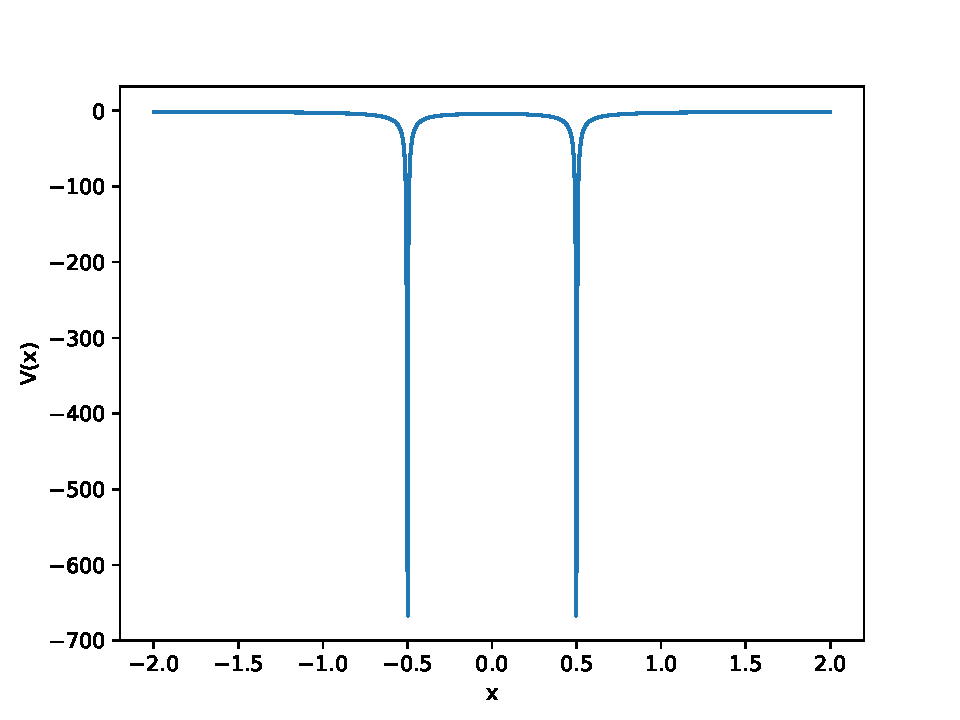
\includegraphics[width=0.7\linewidth]{Images/graph_of_potential}
					\caption[]{Rascunho do potencial $V(x)$}
					\label{fig:graphofpotential}
				\end{figure}
			\end{multianswer}

			% Part 2
			\item If the two protons are very far apart, $r \gg l$, the electron is either localized near the proton on the right (the state $\left|\varphi_{1}\right\rangle$ ), or near the proton on the left (the state $\left|\varphi_{2}\right\rangle$ ). We assume that these states both correspond to the ground state of the hydrogen atom of energy
			$$
			E_{0}=-\frac{1}{2} \frac{m_{\mathrm{e}} e^{4}}{\hbar^{2}}=-\frac{e^{2}}{2 a_{0}}
			$$
			where $m_{\mathrm{e}}$ is the electron mass and $a_{0}$ is the Bohr radius: $a_{0}=\hbar^{2} / m_{\mathrm{e}} e^{2}$. What is the relevant length scale $l$ in the relation $r \gg l$ ?
			\begin{multianswer}
				Somos capazes de distingui-los como átomos separados se $r\geq a_0$, que é o raio de bohr, o raio atômico do hidrogênio. Assim, a distância relevante é $l=a_0$. 				
			\end{multianswer}

			% Part 3
			\item We shall treat the ion $\mathrm{H}_{2}^{+}$as a two-level system with basis states $\left\{\left|\varphi_{1}\right\rangle,\left|\varphi_{2}\right\rangle\right\}$ and $\left\langle\varphi_{i} \mid \varphi_{j}\right\rangle=\delta_{i j}$. Justify the following form of the Hamiltonian with the choice $A>0$ :
			$$
			H=\left(\begin{array}{cc}
				E_{0} & -A \\
				-A & E_{0}
			\end{array}\right)
			$$
			What are the eigenstates $\left|\chi_{+}\right\rangle$and $\left|\chi_{-}\right\rangle$of $H$ and the corresponding energies $E_{+}$and $E_{-}$, $E_{+}<E_{-}$? Qualitatively sketch the wave functions $\chi_{ \pm}(x)=\left\langle x \mid \chi_{ \pm}\right\rangle$of the electron on the $x$ axis.
			\begin{multianswer}
				As energia de ambos os estados são $E_0$, portanto é esperado que as diagonais sejam compostas por $E_0$. Ademais, é necessário introduzir uma perturbação simétrica, convenientemente parametrizada por $-A$ com $A>0$. Assim, a forma da hamiltoniana é natural. Os autovalores são:
				\be
					E_\mp = E_0 \pm A
				\ee
				Os autovetores são dados por:
				\bea
					E_0 a_+ -Ab_+ &=& (E_0 - A)a_+ \\
					Ab_+ &=& Aa_+ \\
					b_+ &=& a_+
				\eea
				Logo, uma escolha normalizada é
				\be
					\ket{\chi_+} = 
					\f{1}{\sqrt{2}}
					\begin{pmatrix}
						1 \\
						1 \\
					\end{pmatrix} 
					=
					\f{\ket{\phi_1} + \ket{\phi_2}}{\sqrt{2}}
				\ee
				Analogamente,
				\be
				\ket{\chi_-} = 
				\f{1}{\sqrt{2}}
				\begin{pmatrix}
					1 \\
					-1 \\
				\end{pmatrix}
				=
				\f{\ket{\phi_1} - \ket{\phi_2}}{\sqrt{2}}
				\ee
				Evidentemente, projetar na base das posições resulta em
				\bea
					\chi_+(x) &=& \f{\phi_1(x) + \phi_2(x)}{\sqrt{2}} \\
					\chi_+(x) &=& \f{\phi_1(x) - \phi_2(x)}{\sqrt{2}} 
				\eea
				Sendo $\phi_1(x), \phi_2(x)$ soluções das equação de Schrödinger para o caso $n=1$ centrados em diferentes pontos, teremos
				\bea
					\chi_+(x) &=& \f{e^{-|x-r/2|/a_0} + e^{-|x+r/2|/a_0}}{\sqrt{2\pi} a_0^{3/2}} \\
					\chi_+(x) &=& \f{e^{-|x-r/2|/a_0} - e^{-|x+r/2|/a_0}}{\sqrt{2\pi} a_0^{3/2}}
				\eea
				com o gráfico da Fig.(\ref{fig:graphofwavefunc}).
				\begin{figure}
					\centering
					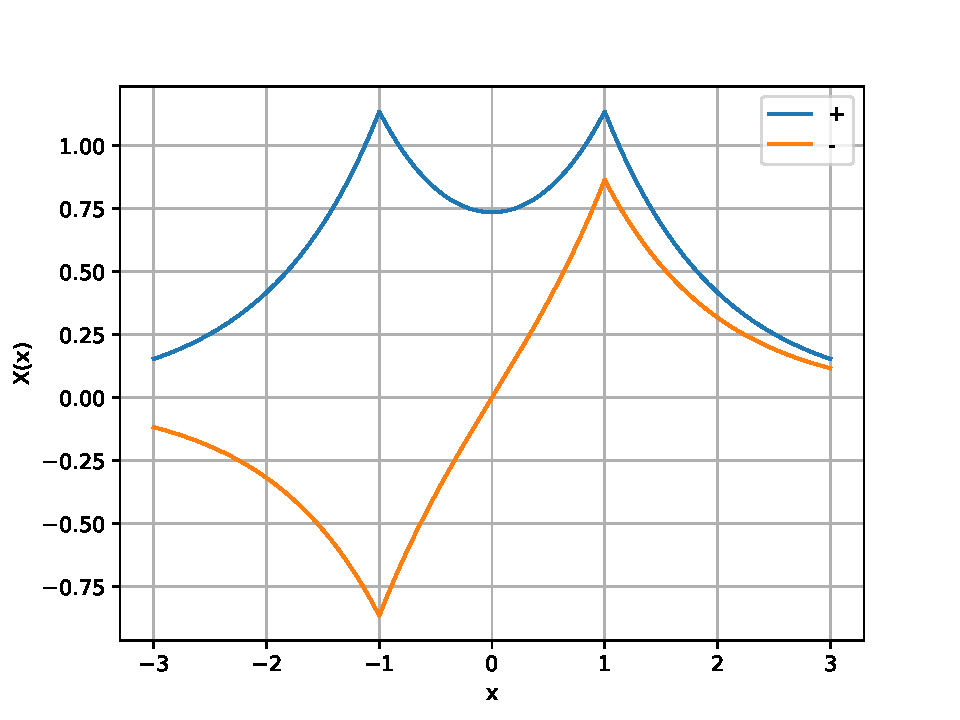
\includegraphics[width=0.7\linewidth]{Images/graph_of_wavefunc}
					\caption{Gráfico não-normalizado das funções de onda $\chi_+(x)$ e $\chi_-(x)$.}
					\label{fig:graphofwavefunc}
				\end{figure}
			\end{multianswer}
		
			% Part 4
			\item The parameter $A$ is a function of the distance $r$ between the protons, $A(r)$. Justify the fact that $A$ is an increasing function of $r$ and $\lim _{r \rightarrow \infty} A(r)=0$. The electron energy is then a function of $r, E_{ \pm}(r)$
			\begin{multianswer}
				Quanto mais distantes os prótons estiverem, menor será sua interação. Quando estiverem em $r\geq a_0$, o elétron já estará bem localizado em apenas um deles com energia $\approx E_0$. Assim, é natural que $A(r)$ decreça conforme $r$ cresce. No limite que $r\to\infty$, não há definitivamente nenhuma interação entre os prótons e temos apenas um átomo de hidrogênio. Assim, obviamente, $E\pm=E_\pm(r)=E_0-A(r)$. 
			\end{multianswer}
			
			% Part 5
			\item Show that the total energy of the ion $E_{ \pm}^{\prime}(r)$ must contain an additional term $+e^{2} / r$. What is the physical origin of this term?
			\begin{multianswer}
				No limite em que $r\to0$, precisamos ter que a energia explode para infinito, pois estamos juntando os dois prótons. Assim, precisamos de um termo $\sim r^{-n}$. É natural adicionar
				\be
					\f{e^2}{r}
				\ee
				pois esse é o termo repulsivo entre os dois prótons. 
			\end{multianswer}
			
			% Part 6
			\item We parametrize $A(r)$ as
			$$
			A(r)=c e^{2} \exp \left(-\frac{r}{b}\right)
			$$
			where $b$ is a length and $c$ an inverse length. Give the expression for the two energy levels $E_{+}^{\prime}$ and $E_{-}^{\prime}$ of the ion. Let
			$$
			\Delta E(r)=E_{+}^{\prime}(r)-E_{0}
			$$
			be the energy difference between the ground state of the ion and that of the hydrogen atom. Show that $\Delta E(r)$ can pass through a minimum at a value $r=r_{0}$ and derive the expression
			$$
			\Delta E\left(r_{0}\right)=\frac{e^{2}}{r_{0}}\left(1-\frac{b}{r_{0}}\right)
			$$
			What condition must hold for $b$ and $r_{0}$ in order for the ion $\mathrm{H}_{2}^{+}$to be a bound state?
			\begin{multianswer}
				Ora, a expressão de $\Delta E(r)$ é
				\be
					\Delta E(r) = -ce^2 e^{-r/b} + \f{e^2}{r}
				\ee
				Essa função explode para $r\to0$ e para $r\to\infty$, então, como é contínua no intervalo $(0, \infty)$, pelo teorema do valor intermediário, precisa existir $r_0\in(0, \infty)$ que minimiza ela. Derivando e igualando a zero para encontrar o mínimo:
				\bea
					-ce^2 e^{-r_0/b} \l(\f{-1}{b}\r) - \f{e^2}{2r_0^2} &=& 0 \\
					e^{-r_0/b} &=& \f{b}{2c r_0^2}
				\eea
				Ora, substituindo isso na expressão original, obtemos
				\be
				\Delta E(r_0) = \frac{e^{2}}{r_{0}}\left(1-\frac{b}{r_{0}}\right)
				\ee
				que é a expressão desejada. Para que esse seja um estado ligado, precisamos que $\Delta E(r_0) < 0$. Portanto, temos a condição $b/r_0 > 1$. 
			\end{multianswer}
			
			% Part 7
			\item The experimental values are $r_{0} \simeq 2 a_{0}$ and $\Delta E\left(r_{0}\right) \simeq E_{0} / 5=-e^{2} / 10 a_{0}$. Compute $b$ and $c$ as functions of $a_{0}$.
			\begin{multianswer}[true]
				Usanos os valores dados:
				\bea
					\f{e^2}{2a_0}\l( 1 - \f{b}{2a_0}\r) &=& \f{-e^2}{10a_0} \\
					1-\f{b}{2a_0} &=& -\f{1}{5} \\
					\f{b}{2a_0} &=& \f{6}{5} \\
					b &=& \f{12a_0}{5}
				\eea
				Por outro lado,
				\bea
					-ce^2e^{-r_0/b} + \f{e^2}{r_0} &=& -\f{e^2}{10a_0} \\
					-ce^{-5/6} + \f{1}{2a_0} &=& -\f{1}{10a_0} \\
					c &=& \f{3e^{5/6}}{5a_0}
				\eea
			\end{multianswer}
		\end{exercises}
	\end{exercise}
	
	\begin{exercise}[5.5.6 - The rotating-wave approximation in NMR]
		\begin{exercises}
			\item Instead of the rotating field of (5.22), we shall use a field $\vec{B}_{1}(t)$ parallel to $O x$ :
			$$
			\vec{B}_{1}(t)=2 B_{1} \hat{x} \cos (\omega t-\phi) .
			$$
			We define the state vector $|\tilde{\varphi}(t)\rangle$ in the rotating frame with angular velocity $\omega$ as
			$$
			|\tilde{\varphi}(t)\rangle=\exp \left[-\frac{i \omega \sigma_{z} t}{2}\right]|\varphi(t)\rangle \quad|\tilde{\varphi}(t=0)\rangle=|\varphi(t=0)\rangle .
			$$
			Why can one call $|\tilde{\varphi}(t)\rangle$ the state vector in the rotating frame? Show that the time evolution of $|\tilde{\varphi}(t)\rangle$ is governed by a Hamiltonian $\tilde{H}(t)$
			$$
			\mathrm{i} \hbar \frac{\mathrm{d}|\tilde{\varphi}\rangle}{\mathrm{d} t}=\tilde{H}(t)|\tilde{\varphi}(t)\rangle
			$$
			where
			$$
			\tilde{H}(t)=\exp \left[-\frac{\mathrm{i} \omega \sigma_{z} t}{2}\right] H(t) \exp \left[\frac{\mathrm{i} \omega \sigma_{z} t}{2}\right]
			$$
			More generally, for any operator $A(t)$, we have in the rotating frame
			$$
			\tilde{A}(t)=\exp \left[-\frac{\mathrm{i} \omega \sigma_{z} t}{2}\right] A(t) \exp \left[\frac{\mathrm{i} \omega \sigma_{z} t}{2}\right]
			$$
			\begin{multianswer}
				
			\end{multianswer}
			
			
			
		\end{exercises}
		
	\end{exercise}
	

\end{document}
